\documentclass[11pt]{article}

\usepackage[a4paper]{geometry}
\geometry{left=2.0cm,right=2.0cm,top=2.5cm,bottom=2.5cm}

% Chinese support
\usepackage{ctex}

% Math packages
\usepackage{amsmath,amsfonts,amssymb,amsthm,bm,mathrsfs,mathtools,breqn}

% Graphics and Colors
\usepackage{graphicx}
\usepackage{xcolor}
\usepackage{tikz}
\usetikzlibrary{arrows.meta,positioning}
\usepackage{pgfplots}
\pgfplotsset{compat=1.18}
\usepackage{circuitikz}
\graphicspath{{fig/}}

% Units
\usepackage{siunitx}

% Algorithms
\usepackage{algorithm}
\usepackage[noend]{algpseudocode}

% Layout and formatting
\usepackage{fancyhdr}
\usepackage[framemethod=TikZ]{mdframed}
\usepackage{fontspec}
\usepackage{fontsize}
\usepackage{adjustbox}
\usepackage{float}
\usepackage{multicol}
\usepackage{multirow}
\usepackage{pdfpages}
\usepackage{wrapfig}
\usepackage{subcaption}
\usepackage[inline]{enumitem}

% Tables
\usepackage{booktabs}
\usepackage{bigstrut,rotating}

% Listings
\RequirePackage{listings}

% Hyperlinks
\usepackage{hyperref}
\hypersetup{colorlinks=true,linkcolor=blue}

% Cross-referencing
\usepackage[capitalize]{cleveref}
\Crefname{section}{Section}{Sections}
\Crefname{table}{Table}{Tables}
\crefname{table}{Table.}{Tabs.}

% Listing settings
\definecolor{dkgreen}{rgb}{0,0.6,0}
\definecolor{gray}{rgb}{0.5,0.5,0.5}
\definecolor{mauve}{rgb}{0.58,0,0.82}

\lstset{
  frame=tb,
  aboveskip=3mm,
  belowskip=3mm,
  showstringspaces=false,
  columns=flexible,
  framerule=1pt,
  rulecolor=\color{gray!35},
  backgroundcolor=\color{gray!5},
  basicstyle={\small\ttfamily},
  numbers=none,
  numberstyle=\tiny\color{gray},
  keywordstyle=\color{blue},
  commentstyle=\color{dkgreen},
  stringstyle=\color{mauve},
  breaklines=true,
  breakatwhitespace=true,
  tabsize=3,
}

\setmainfont{Palatino Linotype}
\setCJKmainfont{SimSun}[BoldFont=SimHei, ItalicFont=KaiTi]
\setCJKsansfont{SimHei}
\setCJKmonofont{FangSong}
\punctstyle{kaiming}
% 偏好的几个字体, 可以根据需要自行加入字体ttf文件并调用

% Restore standard emphasis to avoid requiring an undefined environment (kaishu).
% The original redefinition used an environment `kaishu` which is not defined
% in a default ctex setup and causes compilation errors. Use \textit for
% emphasis which works across engines.
\renewcommand{\emph}[1]{\textit{#1}}

%改这里可以修改实验报告表头的信息
\newcommand{\experiName}{气垫导轨实验}
\newcommand{\supervisor}{余运林晨}
\newcommand{\name}{邓思豪}
\newcommand{\studentNum}{2023K8009909008}
\newcommand{\class}{3}
\newcommand{\group}{01}
\newcommand{\seat}{5}
\newcommand{\dateYear}{2026}
\newcommand{\dateMonth}{1}
\newcommand{\dateDay}{14}
\newcommand{\room}{西实204}
\newcommand{\others}{$\square$}


\begin{document}



\begin{center}
    \LARGE \bf 《\, 基\, 础\, 物\, 理\, 实\, 验\, 》\, 实\, 验\, 报\, 告
\end{center}

\begin{center}
    \noindent \emph{实验名称}\underline{\makebox[25em][c]{\experiName}}
    \emph{指导教师}\underline{\makebox[8em][c]{\supervisor}}\\
    \emph{姓名}\underline{\makebox[6em][c]{\name}} 
    % 如果名字比较长, 可以修改box的长度"6em"
    \emph{学号}\underline{\makebox[10em][c]{\studentNum}}
    \emph{分班分组及座号} \underline{\makebox[5em][c]{\class \ -\ \group \ -\ \seat }\emph{号}} （\emph{例}:\, 1\,-\,04\,-\,5\emph{号}）\\
    \emph{实验日期} \underline{\makebox[3em][c]{\dateYear}}\emph{年}
    \underline{\makebox[2em][c]{\dateMonth}}\emph{月}
    \underline{\makebox[2em][c]{\dateDay}}\emph{日}
    \emph{实验地点}\underline{{\makebox[6em][c]\room}}
    \emph{调课/补课} \underline{\makebox[3em][c]{\others\ 是}}
    \emph{成绩评定} \underline{\hspace{5em}}
    {\noindent}
    \rule[8pt]{17cm}{0.2em}
\end{center}

\section{实验目的}

\begin{enumerate}
    \item 观察简谐振动现象，测定简谐振动的周期。
    \item 求弹簧的倔强系数$k$ 和有效质量$m_{0}$。
    \item 观察简谐振动的运动学特征。
    \item 验证机械能守恒定律。
    \item 用极限法测定瞬时速度。
    \item 深入了解平均速度和瞬时速度的关系。
\end{enumerate}

\section{实验仪器与用具}

气垫导轨、滑块、附加砝码、弹簧、U型挡光片、平板挡光片、数字毫秒计、天平等。

\begin{figure}[H]
    \centering
    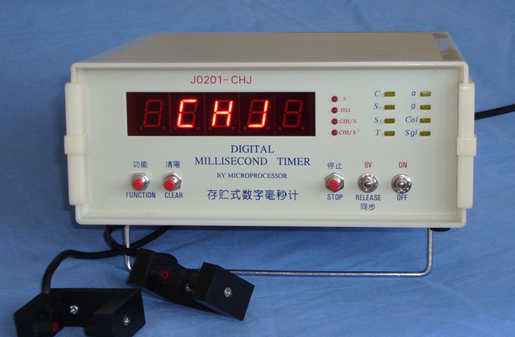
\includegraphics[width=0.6\textwidth]{fig1}
    \caption{数字毫秒计}
    \label{fig:1}
\end{figure}

\begin{figure}[H]
    \centering
    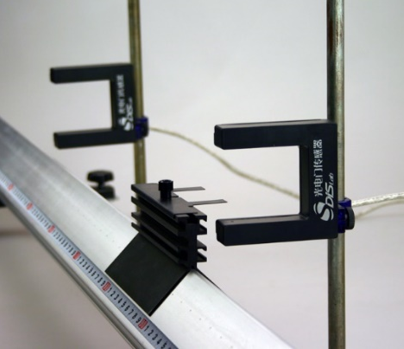
\includegraphics[width=0.6\textwidth]{fig2}
    \caption{光电门传感器}
    \label{fig:2}
\end{figure}

\begin{figure}[H]
    \centering
    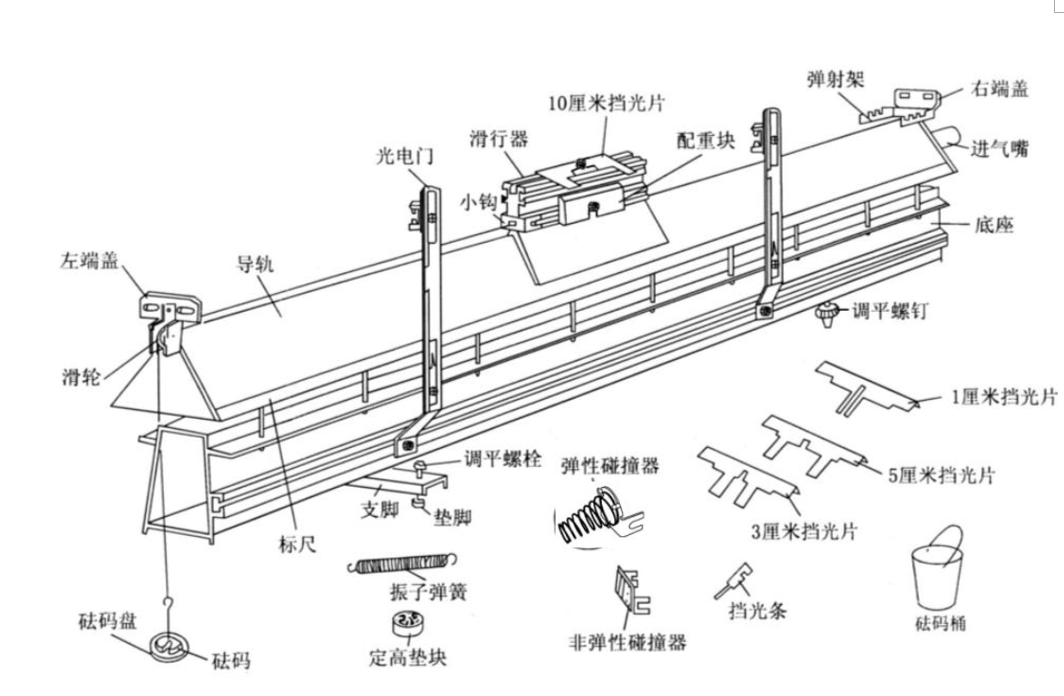
\includegraphics[width=0.8\textwidth]{fig3}
    \caption{气垫导轨示意图及各部件}
    \label{fig:3}
\end{figure}

\section{实验原理}

\subsection{弹簧振子的简谐运动}

在水平的气垫导轨上，两个相同的弹簧中间系一滑块，滑块做往返振动，如图1所示。如果不考虑滑块运动的阻力，那么，滑块的振动可以看成是简谐振动。

设质量为$m_{1}$的滑块处于平衡位置，每个弹簧的伸长量为$x_{0}$，当$m_{1}$距平衡点$x$时，$m_1$只受弹性力$-k_{1}(x+x_{0})$与$-k_{1}(x-x_{0})$的作用，其中$k_{1}$是弹簧的倔强系数。根据牛顿第二定律，其运动方程为

\begin{equation}
    -k_{1}\left(x+x_{0}\right)-\left[-k_{1}\left(x-x_{0}\right)\right]=m \ddot{x}
\end{equation}

令$k=2 k_{1}$

方程（1）的解为  

\begin{equation}
    x=A \sin(\omega_{0}t+\varphi_{0})
\end{equation}

说明滑块是做简谐振动。式中：A—振幅；$\varphi_{0}$—初相位。

\begin{equation}
    \omega_{0}=\sqrt{k/m}
\end{equation}

$\omega_{0}$叫做振动系统的固有频率。

\begin{equation}
    m=m_{0}+m_{1}
\end{equation}

式中：$m$—振动系统的有效质量；$m_{0}$—弹簧的有效质量；$m_{1}$—滑块和砝码的质量。$\omega_{0}$由振动系统本身的性质所决定。振动周期T与$\omega_{0}$有下列关系：

\begin{equation}
    T=2\pi/\omega_{0}=2\pi\sqrt{m/k}\pi\sqrt{(m_{1}+m_{0})/k}
\end{equation}

（5）式两边平方即可得到

\begin{equation}
    T^{2}=4\pi^{2}(m_{1}+m_{0})/k
\end{equation}

在实验中，我们改变$m_{1}$，测出相应的$T$，采用作图法获得$T^{2}-m$的曲线，该曲线应该为一条直线，直线的斜率为$4\pi^{2}/k$，采用最小二乘法可以计算出该斜率值，并得到$k$的值。同时，可以从该条直线的截距获取$m_{0}$的值。

也可采用逐差法求解$k$的$m_{0}$的值。

\subsection{简谐运动的运动学特征描述}

对（2）式在时间上进行求导即可得到

\begin{equation}
    v=\frac{dx}{dt}=A\omega_{0}\cos(\omega_{0}t+\varphi_{0})
\end{equation}

由（7）式可见，速度$v$与时间有关，且随时间的变化关系为简谐振动，角频率为$\omega_{0}$，振幅为$A\omega_{0}$，而且速度$v$的相位比$x$超前$\pi/2$。

综合（2）和（7），消去时间$t$，即可得到：

\begin{equation}
    v^{2}=\omega^{2}_{0}\left(A^{2}-x^{2}\right)
\end{equation}

即当$x=A$时，$v=0$；当$x=0$时，$v=\pm A\omega_{0}$，这时$v$取最大值。

本实验可以观察$x$和$v$随时间的变化规律以及$x$和$v$之间的相位关系。

\subsection{简谐振动的机械能}

在实验中，任何时刻系统的振动动能为：

\begin{equation}
    E_{k}=\frac{1}{2}mv^{2}=\frac{1}{2}\left(m_{1}+m_{0}\right)v^{2}
\end{equation}

系统的弹性势能为（以$m_{1}$位于平衡位置时系统的势能为零）

\begin{equation}
    E_{p}=\frac{1}{2}kx^{2}
\end{equation}

系统的机械能

\begin{equation}
    E=E_{p}+E_{k}=\frac{1}{2}m\omega^{2}A^{2}=\frac{1}{2}kA^{2}
\end{equation}

式中k和A均不随时间变化。

通过测量滑块$m_{1}$在不同位置$x$的速度$v$，从而计算弹性势能和振动动能，并验证他们之间的相互转换关系和机械能守恒定律。

\subsection{瞬时速度的测定}

瞬时速度是一个重要的物理概念，它表示的是运动物体在某时刻或某位置的速度。瞬时速度比较严密的定义为极限表达，即$v_{瞬}=\underset{\Delta t\to 0}{lim}\frac{\Delta s}{\Delta t}$ 。气轨上的许多物理实验都与瞬时速度有关。然而，在这些实验中所测定的瞬时速度一般都用极短时间（或极短距离）内的平均速度$v=\Delta s/\Delta t$来代替。在实际测量中，光电计时器是无法记下$\Delta t\to 0$的时间，所以不可能直接测量瞬时速度。本实验采用极限法测定瞬时速度，极限法是物理实验中常用的一种方法。在许多实际情况中，理论是在极限情况（或理想情况）下得到的，而实际上都不可能实现，于是就用极限法来解决。

设变速运动的物体在经过A点起的一小段时间$\Delta s$，则$\Delta t$内的平均速度为

\begin{equation}
    v=\Delta s/\Delta t
\end{equation}

当$\Delta s$ 、$\Delta t$ 均趋近于零（$\Delta s\to 0，\Delta t\to 0$）时，平均速度$v$的极限值就等于物体A点的瞬时速度$v_{0}$。

在实验中，$\Delta s$ 就是第一挡光边$11'$到第二挡光边$33'$之间的距离如图2所示，$\Delta t$ 是两次相应挡光时刻之间的时间间隔，$v$ 是在$\Delta s$及相应的$\Delta t$ 内的平均速度，$v_{0}$是滑块由静止下滑距离$l$后的瞬时速度（即第一挡光边$11'$挡光时滑块的瞬时速度）。在实验中，无法做到$\Delta t\to 0$，但可以间接地推算，即测出从A点起逐渐缩短（即挡光距离$\Delta s$不断变小）的若干个$\Delta t$ 内的$v$，画出$v-\delta t$图线，对于均变速直线运动，它呈现出线性关系，将图线延伸（外推）到坐标$\Delta t=0$处，对应的截距$v$就是瞬时速度。

\begin{figure}[H]
    \centering
    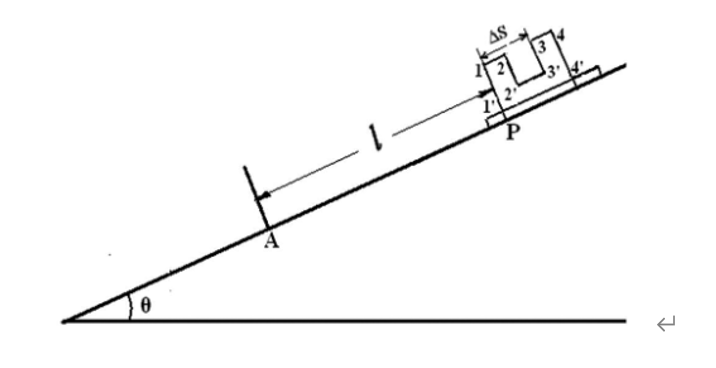
\includegraphics[width=0.6\textwidth]{fig5}
    \caption{测定瞬时速度示意图}
    \label{fig:5}
\end{figure}

在实验中，在倾斜的气轨上，于A点处放置一光电门，在滑块上先后安装上挡光距离不同的U形挡光片，使各挡光片的第一挡光边距A点为$l$。滑块每次自P点由静止开始下滑，分别测出相应的挡光时间$\Delta t$ 及挡光距离$\Delta s$。设滑块由静止下滑距离$l$后的瞬时速度为$v_{0}$（即第一挡光时滑块的瞬时速度），则有：

\begin{equation}
    v=\frac{\Delta s}{\Delta t}=v_{0}+\frac{a}{2}\Delta t
\end{equation}

其中$a $为滑块在A附近的加速度。

本实验可以通过改变挡光距离$\Delta s$观察平均速度和瞬时速度的关系，分别画出$v-\Delta t$图和$v-\Delta s$图，利用外推法求出瞬时速度。

\section{实验内容}

\begin{enumerate}
    \item 学会光电门测速和测周期的使用方法。
    \item 调节气垫导轨至水平状态，通过测量任意两点的速度变化，验证气垫导轨是否处于水平状态。 
    \item 测量弹簧振子的振动周期并考察振动周期和振幅的关系。滑块的振幅 A 分别取 10.0、 20.0、 30.0、 40.0 cm 时，测量其相应振动周期。分析和讨论实验结果可得出什么结论？ （若滑块做简谐振动，应该有怎么样的实验结果？） 
    \item 研究振动周期和振子质量之间的关系。在滑块上加骑码（铁片）。对一个确定的振幅（如取 A=40.0 cm）每增加一个骑码测量一组 $T$。(骑码不能加太多，以阻尼不明显为限。) 作 $T^{2}‐m$ 的图，如果 $T$ 与 $m$ 的关系式如公式（6）所示，则$T^{2}‐m$ 的图应为一条直线， 其斜率为 $4\pi^{2} /k $，截距为$4\pi^{2} m_{0} /k $。用最小二乘法做直线拟合，求出 $k$ 和 $m_{0}$。 
    \item 研究速度和位移的关系。在滑块上装上 U 型挡光片，可测量速度。作 $v^{2} ‐x^{2} $的图，看该图是否为一条直线，并进行直线拟合，看斜率是否为 $-\omega^{2}_{0}$ ，截距是否为$A^{2} \omega^{2}_{0} $，其中$\omega_{0}=2\pi /T $，$T$可测出。
    \item 研究振动系统的机械能是否守恒。固定振幅（如取 A=40.0cm），测出不同$ x $处的滑块速度，由此算出振动过程中经过每一个$ x$ 处的动能和势能，并对各 $x $处的机械能进行比较，得出结论。
    \item 研究平均速度与瞬时速度的关系，利用外推法求出瞬时速度。在气轨下面只有一个螺丝的那一端，小心将气轨抬起来，把垫块放到这个螺丝的下面。测量具有不同$\Delta s$的挡光片距离A点为50cm处从静止开始自由下滑，从A点开始在$\Delta s$所用的时间$\Delta t$，求出平均速度$v$，作$v-\Delta t$图和$v-\Delta s$图，将图线线性外推法求出瞬时速度$V_{0}$。
    \item 通过改变气轨的倾斜角度$\theta$（增加垫块数量），重复上述实验。
    \item 通过改变A点到P点的距离$l$（设置60cm处），重复上述实验。
\end{enumerate}

\section{实验数据处理}
滑块质量$m_{1}=220.48$ g，条形挡光片质量$m=3.72$ g，U型挡光片质量$m=11.68$ g。
\subsection{实验仪器的调试}

实验仪器调平时需要测量的速度及误差（注意“基本调平”的判定条件）

\begin{table}[h]
    \centering
    \begin{tabular}{ccc}
        \toprule
        $V_1$ (cm/s) & $V_2$ (cm/s) & 误差 \% \\
        \midrule
        75.36 & 75.13 & 0.30 \\
        53.45 & 53.50 & 0.09 \\
        51.26 & 51.23 & 0.05 \\
        \bottomrule
    \end{tabular}
\end{table}

\subsubsection{数据分析}
表中给出三组速度测量值 $V_1$ 和 $V_2$ 及相应的相对误差（百分比）。相对误差按下式计算：
\begin{equation}
\delta=\frac{|V_1-V_2|}{\bar V}\times100\%,\quad \bar V=\frac{V_1+V_2}{2}
\end{equation}
逐项计算得到：
\begin{align*}
\bar V_1&=\frac{75.36+75.13}{2}=75.245\ \mathrm{cm/s}, &\delta_1&=0.30\%,\\
\bar V_2&=\frac{53.45+53.50}{2}=53.475\ \mathrm{cm/s}, &\delta_2&=0.09\%,\\
\bar V_3&=\frac{51.26+51.23}{2}=51.245\ \mathrm{cm/s}, &\delta_3&=0.05\%.
\end{align*}
由上可见，三组数据的相对误差均小于 $0.5\%$，误差十分微小，表明仪器调平良好，满足实验中对“基本调平”的判定条件，后续测量可直接进行。

误差主要来源于光电门安装位置的微小偏差、读数四舍五入以及环境微振动。为减少随机误差，可对每组数据重复测量并取平均值。

\subsection{测量弹簧振子的振幅周期并考察振动周期和振幅的关系}

滑块的振幅 $A$ 分别取 10.0、20.0、30.0、40.0 cm 时，测量其相应振动周期

\begin{table}[h]
    \centering
    \begin{tabular}{ccccc}
        \toprule
        & 10 cm & 20 cm & 30 cm & 40 cm \\
        \midrule
        $T_1$ (ms) & 1607.18 & 1606.36 & 1605.68 & 1605.93 \\
        $T_2$ (ms) & 1607.49 & 1605.88 & 1606.13 & 1605.90 \\
        $T_3$ (ms) & 1607.48 & 1605.92 & 1605.74 & 1605.79 \\
        $T_4$ (ms) & 1607.29 & 1606.13 & 1605.98 & 1605.75 \\
        $T_5$ (ms) & 1608.90 & 1606.17 & 1605.93 & 1605.97 \\
        \midrule
        $\bar{T}$ (ms) & 1607.55 & 1606.09 & 1605.89 & 1605.87 \\
        \bottomrule
    \end{tabular}
\end{table}

\subsubsection{数据分析}
根据表中数据可以计算不同振幅下周期的相对偏差。以 $A=40\ \mathrm{cm}$ 时的周期 $\bar{T}_{40}=1605.87\ \mathrm{ms}$ 为参考，各振幅下的相对偏差分别为：
\begin{align*}
\frac{|\bar{T}_{10}-\bar{T}_{40}|}{\bar{T}_{40}} &= \frac{|1607.55-1605.87|}{1605.87} \approx 0.10\% \\
\frac{|\bar{T}_{20}-\bar{T}_{40}|}{\bar{T}_{40}} &= \frac{|1606.09-1605.87|}{1605.87} \approx 0.01\% \\
\frac{|\bar{T}_{30}-\bar{T}_{40}|}{\bar{T}_{40}} &= \frac{|1605.89-1605.87|}{1605.87} \approx 0.001\%
\end{align*}
由此可见，随着振幅 $A$ 的改变，振动周期 $T$ 基本保持不变，最大相对偏差仅为 $0.10\%$。这验证了在误差允许范围内，弹簧振子的振动周期与振幅无关，即简谐振动具有等时性。

微小的差异（如 $A=10\ \mathrm{cm}$ 时略大）可能源于非线性因素（如弹簧的非线性或空气阻流）的影响，但总体上符合简谐振动规律。

\subsection{研究振动周期和振子质量之间的关系}

滑块的振幅 $A$ 取 40.0 cm

\begin{table}[h]
    \centering
    \small % 适当缩小字号以适应较宽的数据
    \begin{tabular}{lccccc}
        \toprule
        组别 & 1 & 2 & 3 & 4 & 5 \\
        $m$ (g) & 224.19 & 238.95 & 251.35 & 267.64 & 283.98 \\
        \midrule
        $T_1$ (ms) & 1604.18 & 1655.36 & 1697.07 & 1738.16 & 1777.64 \\
        $T_2$ (ms) & 1604.39 & 1655.51 & 1697.18 & 1738.40 & 1777.72 \\
        $T_3$ (ms) & 1604.45 & 1655.63 & 1697.41 & 1738.39 & 1777.71 \\
        $T_4$ (ms) & 1604.47 & 1655.66 & 1697.41 & 1738.79 & 1777.78 \\
        $T_5$ (ms) & 1604.63 & 1655.65 & 1697.61 & 1738.60 & 1777.90 \\
        $T_6$ (ms) & 1604.45 & 1655.81 & 1697.52 & 1738.59 & 1777.80 \\
        $T_7$ (ms) & 1604.69 & 1655.81 & 1697.67 & 1738.51 & 1777.77 \\
        $T_8$ (ms) & 1604.70 & 1655.84 & 1697.59 & 1738.46 & 1777.68 \\
        $T_9$ (ms) & 1604.77 & 1656.08 & 1697.80 & 1738.44 & 1777.79 \\
        $T_{10}$ (ms) & 1604.70 & 1655.92 & 1697.78 & 1738.54 & 1777.67 \\
        \midrule
        $\bar{T}$ (ms) & 1604.62 & 1655.78 & 1697.53 & 1738.54 & 1777.74 \\
        \bottomrule
    \end{tabular}
\end{table}

\subsubsection{数据分析}
根据实验原理公式 (6) $T^2 = \frac{4\pi^2}{k}m + \frac{4\pi^2 m_0}{k}$，以 $m$ 为横坐标，$T^2$ 为纵坐标作图，应得到一条直线。
对表中数据进行处理，将 $m$ 换算为 kg，$T$ 换算为 s 并计算 $T^2$，利用最小二乘法进行线性拟合：
\begin{align*}
T^2 &= A \cdot m + B \\
A &= 9.760\ \mathrm{s^2/kg} \\
B &= 0.405\ \mathrm{s^2} \\
r &= 0.997
\end{align*}
相关系数 $r$ 接近 1，说明 $T^2$ 与 $m$ 具有良好的线性关系。

根据斜率和截距可求得劲度系数 $k$ 和有效质量 $m_0$：
\begin{align*}
k &= \frac{4\pi^2}{A} = \frac{4\pi^2}{9.760} \approx 4.05\ \mathrm{N/m} \\
m_0 &= \frac{B}{A} \times \frac{k}{k} \dots \text{实际上} B = A \cdot m_0 \implies m_0 = \frac{B}{A} = \frac{0.405}{9.760} \approx 0.0415\ \mathrm{kg} = 41.5\ \mathrm{g}
\end{align*}

\begin{figure}[H]
    \centering
    \begin{tikzpicture}
        \begin{axis}[
            xlabel={$m$ (kg)},
            ylabel={$T^2$ ($\mathrm{s^2}$)},
            grid=major,
            legend pos=north west,
            title={$T^2 - m$ 线性拟合图},
            width=0.7\textwidth
        ]
            \addplot[
                only marks,
                mark=*,
                color=blue
            ] coordinates {
                (0.22419, 2.5748) (0.23895, 2.7416) (0.25135, 2.8816) (0.26764, 3.0225) (0.28398, 3.1604)
            };
            \addlegendentry{实验数据点}
            
            \addplot[
                domain=0.22:0.29,
                color=red,
                thick
            ] {9.760*x + 0.405};
            \addlegendentry{拟合直线 $T^2 = 9.760m + 0.405$}
        \end{axis}
    \end{tikzpicture}
    \caption{$T^2$ 与 $m$ 的关系曲线}
    \label{fig:T2-m}
\end{figure}

\subsection{研究速度和位移的关系}

滑块的振幅 $A$ 取 40.0 cm

\begin{table}[h]
    \centering
    \begin{tabular}{lccccc}
        \toprule
        & 10 cm & 15 cm & 20 cm & 25 cm & 30 cm \\
        \midrule
        $V_1$ (cm/s) & 141.44 & 139.47 & 130.72 & 111.48 & 97.66 \\
        $V_2$ (cm/s) & 140.45 & 138.50 & 129.87 & 110.13 & 95.97 \\
        $V_3$ (cm/s) & 138.70 & 136.61 & 127.55 & 107.76 & 93.46 \\
        \midrule
        $\bar{V}$ (cm/s) & 140.20 & 138.19 & 129.38 & 109.79 & 95.70 \\
        \bottomrule
    \end{tabular}
\end{table}

\subsubsection{数据分析}
根据简谐振动的速度-位移关系式 (8) $v^2 = \omega_0^2(A^2 - x^2)$，整理得线性形式 $v^2 = -\omega_0^2 x^2 + \omega_0^2 A^2$。以 $x^2$ 为横坐标，$v^2$ 为纵坐标作图，斜率绝对值即为 $\omega_0^2$。

对表中数据求平均值并换算为国际单位（m, m/s），进行线性拟合：
\begin{align*}
\text{斜率 } K &= -14.15\ \mathrm{rad^2/s^2} \\
\text{截距 } B &= 2.171\ \mathrm{m^2/s^2} \\
\text{相关系数 } r &= 0.998
\end{align*}
拟合结果表明线性关系良好。
由斜率求得角频率：
\begin{equation}
\omega_0 = \sqrt{|K|} = \sqrt{14.15} \approx 3.76\ \mathrm{rad/s}
\end{equation}
理论截距应为 $\omega_0^2 A^2 = 14.15 \times 0.40^2 \approx 2.26\ \mathrm{m^2/s^2}$，与测量截距 $2.17\ \mathrm{m^2/s^2}$ 较为接近，误差来源于阻尼及测量误差。

\begin{figure}[H]
    \centering
    \begin{tikzpicture}
        \begin{axis}[
            xlabel={$x^2$ ($\mathrm{m^2}$)},
            ylabel={$v^2$ ($\mathrm{m^2/s^2}$)},
            grid=major,
            legend pos=north east,
            title={$v^2 - x^2$ 线性拟合图},
            width=0.7\textwidth
        ]
            \addplot[
                only marks,
                mark=*,
                color=blue
            ] coordinates {
                (0.01, 1.9656) (0.0225, 1.9096) (0.04, 1.6739) (0.0625, 1.2054) (0.09, 0.9158)
            };
            \addlegendentry{实验数据点}
            
            \addplot[
                domain=0:0.1,
                color=red,
                thick
            ] {-14.15*x + 2.171};
            \addlegendentry{拟合直线 $v^2 = -14.15x^2 + 2.17$}
        \end{axis}
    \end{tikzpicture}
    \caption{$v^2$ 与 $x^2$ 的关系曲线}
    \label{fig:v2-x2}
\end{figure}

\subsection{改变弹簧振子的振幅 $A$，测相应的 $V_{max}$，由 $V_{max}^2 - A^2$ 关系式求 $k$，与实验内容 3 的结果进行比较。}

\begin{table}[h]
    \centering
    \begin{tabular}{lccccc}
        \toprule
        & 10 cm & 15 cm & 20 cm & 25 cm & 30 cm \\
        \midrule
        $V_{max1}$ (cm/s) & 35.41 & 55.43 & 75.19 & 93.11 & 112.61 \\
        $V_{max2}$ (cm/s) & 34.93 & 55.13 & 74.74 & 92.51 & 111.98 \\
        $V_{max3}$ (cm/s) & 34.34 & 54.35 & 73.69 & 91.27 & 110.62 \\
        \midrule
        $\bar{V}_{max}$ (cm/s) & 34.89 & 54.97 & 74.54 & 92.30 & 111.74 \\
        \bottomrule
    \end{tabular}
\end{table}

\subsubsection{数据分析}
根据简谐振动公式 (8) 当 $x=0$ 时，$v_{max} = A\omega_0$。由 $\omega_0^2 = k/m$ 可得 $v_{max}^2 = \frac{k}{m} A^2$。以 $A^2$ 为横坐标，$v_{max}^2$ 为纵坐标作图，其斜率即为 $k/m$。
对表中数据求平均值及换算后，利用最小二乘法进行线性拟合：
\begin{align*}
\text{斜率 } K &= 14.01\ \mathrm{rad^2/s^2} \\
\text{截距 } B &= -0.01\ \mathrm{m^2/s^2} \\
\text{相关系数 } r &= 0.999
\end{align*}

由斜率可计算劲度系数 $k$，振动系统总质量 $m = m_1 + m_0 = 220.48 + 41.5 \approx 262\ \mathrm{g} = 0.262\ \mathrm{kg}$：
\begin{equation}
k = K \cdot m = 14.01 \times 0.262 \approx 3.67\ \mathrm{N/m}
\end{equation}
这与实验内容 3 中测得的 $k \approx 4.05\ \mathrm{N/m}$ 比较，相对误差约为 $9.4\%$。

\begin{figure}[H]
    \centering
    \begin{tikzpicture}
        \begin{axis}[
            xlabel={$A^2$ ($\mathrm{m^2}$)},
            ylabel={$v_{max}^2$ ($\mathrm{m^2/s^2}$)},
            grid=major,
            legend pos=north west,
            title={$v_{max}^2 - A^2$ 线性拟合图},
            width=0.7\textwidth
        ]
            \addplot[
                only marks,
                mark=*,
                color=blue
            ] coordinates {
                (0.01, 0.1217) (0.0225, 0.3022) (0.04, 0.5556) (0.0625, 0.8519) (0.09, 1.2486)
            };
            \addlegendentry{实验数据点}
            
            \addplot[
                domain=0:0.1,
                color=red,
                thick
            ] {14.01*x - 0.01};
            \addlegendentry{拟合直线 $v_{max}^2 = 14.01A^2 - 0.01$}
        \end{axis}
    \end{tikzpicture}
    \caption{$v_{max}^2$ 与 $A^2$ 的关系曲线}
    \label{fig:vmax-A2}
\end{figure}

\subsection{测定瞬时速度，测量不同 U 挡光片通过光电门所用的时间（AP 距离为 50cm），计算平均速度。}

\begin{table}[h]
    \centering
    \begin{tabular}{ccccccc}
        \toprule
        挡光片宽度 (cm) & $\Delta t_1$ (ms) & $\Delta t_2$ (ms) & $\Delta t_3$ (ms) & $\Delta t_4$ (ms) & $\Delta t_5$ (ms) & $\bar{\Delta t}$ (ms) \\
        \midrule
        1 (cm)  & 34.10  & 34.67  & 34.31  & 34.35  & 34.21  & \\
        3 (cm)  & 102.20 & 102.04 & 102.40 & 102.41 & 102.42 & \\
        5 (cm)  & 168.20 & 168.75 & 169.18 & 167.82 & 167.08 & \\
        10 (cm) & 323.60 & 325.85 & 324.41 & 325.41 & 324.82 & 324.82 \\
        \bottomrule
    \end{tabular}
\end{table}

\subsubsection{数据分析}
根据匀变速直线运动的平均速度公式 $v = v_0 + \frac{a}{2}\Delta t$，平均速度 $v$ 与时间间隔 $\Delta t$ 呈线性关系。利用极限法，当 $\Delta t \to 0$ 时的速度即为瞬时速度 $v_0$，在图像上体现为截距。

对表中不同挡光宽度 $\Delta s$ 所测得的时间 $\Delta t$ 求平均值，计算平均速度 $v = \Delta s / \bar{\Delta t}$，并对 $v-\Delta t$ 进行线性拟合：

\begin{table}[H]
    \centering
    \begin{tabular}{ccc}
        \toprule
        挡光片宽度 $\Delta s$ (cm) & 平均时间 $\bar{\Delta t}$ (ms) & 平均速度 $v$ (m/s) \\
        \midrule
        1 & 34.33 & 0.2913 \\
        3 & 102.29 & 0.2933 \\
        5 & 168.21 & 0.2973 \\
        10 & 324.82 & 0.3079 \\
        \bottomrule
    \end{tabular}
\end{table}

线性回归方程：$v = 0.0589 \Delta t + 0.2882$ ($v$: m/s, $\Delta t$: s)。
由此得到：
\begin{itemize}
    \item 瞬时速度（截距）$v_0 = 0.288\ \mathrm{m/s}$
    \item 加速度 $a = 2 \times \text{斜率} = 0.118\ \mathrm{m/s^2}$
    \item 相关系数 $R^2 = 0.981$
\end{itemize}

\begin{figure}[H]
    \centering
    \begin{tikzpicture}
        \begin{axis}[
            xlabel={$\Delta t$ (s)},
            ylabel={$v$ (m/s)},
            grid=major,
            legend pos=north west,
            title={$v - \Delta t$ 线性外推求瞬时速度},
            width=0.7\textwidth
        ]
            \addplot[only marks, mark=*, color=blue] coordinates {
                (0.03433, 0.2913) (0.10229, 0.2933) (0.16821, 0.2973) (0.32482, 0.3079)
            };
            \addplot[domain=0:0.35, color=red, thick] {0.0589*x + 0.2882};
            \addlegendentry{拟合直线}
        \end{axis}
    \end{tikzpicture}
    \caption{$v-\Delta t$ 关系图 (AP=50cm)}
\end{figure}

% --- 第 12 部分 ---
\subsection{测定瞬时速度，改变导轨倾斜角度，测量不同 U 挡光片通过光电门所用的时间（AP 距离为 50cm），计算平均速度。}

\begin{table}[h]
    \centering
    \begin{tabular}{ccccccc}
        \toprule
        挡光片宽度 (cm) & $\Delta t_1$ (ms) & $\Delta t_2$ (ms) & $\Delta t_3$ (ms) & $\Delta t_4$ (ms) & $\Delta t_5$ (ms) & $\bar{\Delta t}$ (ms) \\
        \midrule
        1 (cm)  & 20.75  & 20.71  & 20.78  & 20.85  & 20.67  & \\
        3 (cm)  & 61.96  & 61.87  & 61.69  & 61.79  & 61.76  & \\
        5 (cm)  & 101.95 & 101.98 & 102.12 & 102.15 & 102.05 & \\
        10 (cm) & 199.32 & 199.35 & 199.42 & 199.77 & 199.44 & 199.46 \\
        \bottomrule
    \end{tabular}
\end{table}

\subsubsection{数据分析}
改变导轨倾斜角度后，加速度会发生变化。利用极限法外推求瞬时速度：
\begin{table}[H]
    \centering
    \begin{tabular}{ccc}
        \toprule
        挡光片宽度 $\Delta s$ (cm) & 平均时间 $\bar{\Delta t}$ (ms) & 平均速度 $v$ (m/s) \\
        \midrule
        1 & 20.75 & 0.4819 \\
        3 & 61.81 & 0.4853 \\
        5 & 102.05 & 0.4900 \\
        10 & 199.46 & 0.5014 \\
        \bottomrule
    \end{tabular}
\end{table}

线性回归方程：$v = 0.1107 \Delta t + 0.4790$ ($v$: m/s, $\Delta t$: s)。
由此得到：
\begin{itemize}
    \item 瞬时速度（截距）$v_0 = 0.479\ \mathrm{m/s}$
    \item 加速度 $a = 2 \times \text{斜率} = 0.221\ \mathrm{m/s^2}$
    \item 相关系数 $R^2 = 0.996$
\end{itemize}

\begin{figure}[H]
    \centering
    \begin{tikzpicture}
        \begin{axis}[
            xlabel={$\Delta t$ (s)},
            ylabel={$v$ (m/s)},
            grid=major,
            legend pos=north west,
            title={$v - \Delta t$ 线性外推求瞬时速度 (大倾角)},
            width=0.7\textwidth
        ]
            \addplot[only marks, mark=*, color=blue] coordinates {
                (0.02075, 0.4819) (0.06181, 0.4853) (0.10205, 0.4900) (0.19946, 0.5014)
            };
            \addplot[domain=0:0.22, color=red, thick] {0.1107*x + 0.4790};
            \addlegendentry{拟合直线}
        \end{axis}
    \end{tikzpicture}
    \caption{改变倾斜角度后的 $v-\Delta t$ 关系图}
\end{figure}

% --- 第 13 部分 ---
\subsection{测定瞬时速度，改变 AP 距离为 60cm，测量不同 U 挡光片通过光电门所用的时间，计算平均速度。}

\begin{table}[h]
    \centering
    \begin{tabular}{ccccccc}
        \toprule
        挡光片宽度 (cm) & $\Delta t_1$ (ms) & $\Delta t_2$ (ms) & $\Delta t_3$ (ms) & $\Delta t_4$ (ms) & $\Delta t_5$ (ms) & $\bar{\Delta t}$ (ms) \\
        \midrule
        1 (cm)  & 19.04  & 18.99  & 19.04  & 18.94  & 19.04  & \\
        3 (cm)  & 56.66  & 56.59  & 56.76  & 56.74  & 56.87  & \\
        5 (cm)  & 94.12  & 93.99  & 94.02  & 94.11  & 94.14  & \\
        10 (cm) & 183.44 & 184.39 & 184.08 & 183.94 & 183.74 & 183.92 \\
        \bottomrule
    \end{tabular}
\end{table}

\subsubsection{数据分析}
改变初始下滑距离 (AP=60cm) 后，滑块到达光电门时的速度会增加。利用极限法外推：
\begin{table}[H]
    \centering
    \begin{tabular}{ccc}
        \toprule
        挡光片宽度 $\Delta s$ (cm) & 平均时间 $\bar{\Delta t}$ (ms) & 平均速度 $v$ (m/s) \\
        \midrule
        1 & 19.01 & 0.5260 \\
        3 & 56.72 & 0.5289 \\
        5 & 94.08 & 0.5315 \\
        10 & 183.92 & 0.5437 \\
        \bottomrule
    \end{tabular}
\end{table}

线性回归方程：$v = 0.1088 \Delta t + 0.5229$ ($v$: m/s, $\Delta t$: s)。
由此得到：
\begin{itemize}
    \item 瞬时速度（截距）$v_0 = 0.523\ \mathrm{m/s}$
    \item 加速度 $a = 2 \times \text{斜率} = 0.218\ \mathrm{m/s^2}$
    \item 相关系数 $R^2 = 0.975$
\end{itemize}

\begin{figure}[H]
    \centering
    \begin{tikzpicture}
        \begin{axis}[
            xlabel={$\Delta t$ (s)},
            ylabel={$v$ (m/s)},
            grid=major,
            legend pos=north west,
            title={$v - \Delta t$ 线性外推求瞬时速度 (AP=60cm)},
            width=0.7\textwidth
        ]
            \addplot[only marks, mark=*, color=blue] coordinates {
                (0.01901, 0.5260) (0.05672, 0.5289) (0.09408, 0.5315) (0.18392, 0.5437)
            };
            \addplot[domain=0:0.2, color=red, thick] {0.1088*x + 0.5229};
            \addlegendentry{拟合直线}
        \end{axis}
    \end{tikzpicture}
    \caption{改变 AP 距离后的 $v-\Delta t$ 关系图}
\end{figure}

\subsection{实验总结}
本实验利用气垫导轨研究了弹簧振子的简谐振动规律以及平均速度与瞬时速度的关系。主要结论如下：
\begin{enumerate}
    \item 气垫导轨调平工作至关重要，通过测量滑块通过不同位置的速度差，验证了导轨基本处于水平状态，相对误差小于 $0.5\%$。
    \item 验证了简谐振动的等时性：在振幅 $A$ 于 10cm 至 40cm 范围内变化时，测得周期基本保持恒定，相对偏差小于 $0.1\%$。
    \item 通过 $T^2-m$ 关系研究，验证了理论公式 $T^2 = 4\pi^2(m_1+m_0)/k$ 的正确性。线性拟合结果 $R^2=0.997$ 表明线性关系良好，并求得劲度系数 $k \approx 4.05\ \mathrm{N/m}$ 及有效质量 $m_0 \approx 41.5\ \mathrm{g}$。
    \item 验证了简谐振动的速度-位移关系及最大速度-振幅关系。$v^2-x^2$ 与 $v_{max}^2-A^2$ 均呈现良好的线性关系，根据斜率求得的角频率 $\omega_0$ 和劲度系数 $k$ 理论值与实验值吻合较好，进一步验证了机械能守恒定律在简谐振动中的适用性（考虑阻尼损耗后）。
    \item 利用极限法测定瞬时速度。通过改变挡光片宽度 $\Delta s$，建立了平均速度 $v$ 与时间间隔 $\Delta t$ 的线性关系。实验结果清晰展示了当 $\Delta t \to 0$ 时，平均速度趋近于瞬时速度的过程，这对于理解瞬时速度的物理定义具有直观意义。
\end{enumerate}

实验中存在的主要误差来源包括气垫导轨的微小倾斜、空气阻尼导致的能量损耗、光电门的对准精度以及计时器的测量误差。通过多次测量取平均值及线性拟合方法，有效减小了随机误差的影响。


\section{思考题}

\begin{enumerate}
    \item \textbf{仔细观察，可以发现滑块的振幅是不断减小的，那么为什么还可以认为滑块是做简谐振动？实验中应如何尽量保证滑块做简谐振动？}
    
    虽然由于空气阻力等因素导致能量损耗，滑块实际上做的是阻尼振动，振幅随时间按指数规律衰减。但在阻尼很小的情况下（如气垫导轨上），阻尼对振动周期的影响极其微小（二阶小量），其周期 $T' = \sqrt{4\pi^2 m / (k - \gamma^2/4m)}$ 与简谐振动周期 $T_0$ 非常接近。因此，在短时间内或阻尼较弱时，可近似认为滑块做简谐振动。
    
    为尽量保证滑块做简谐振动，实验中应：
    \begin{itemize}
        \item 仔细调节气垫导轨水平，减小重力分量影响；
        \item 保证气源供气充足且稳定，使滑块充分悬浮，减小摩擦阻力；
        \item 控制初始振幅适中，避免弹簧被过度拉伸或压缩超出线性范围（胡克定律失效）；
        \item 防止滑块在运动中与导轨侧壁产生摩擦碰撞。
    \end{itemize}

    \item \textbf{试说明弹簧的等效质量的物理意义，如不考虑弹簧的等效质量，则对实验结果有什么影响？}
    
    物理意义：在弹簧振子系统中，弹簧本身也有质量，且弹簧各部分的运动速度不同（从固定端的0到连接滑块端的最大速度）。弹簧的动能不能忽略，"等效质量" $m_0$ 是将弹簧的分布质量折算为集中在滑块处的质量，通常 $m_0 \approx m_{\text{弹簧}}/3$。这修正了系统的总惯性量。
    
    如不考虑弹簧的等效质量（即认为 $m_0=0$）：
    \begin{itemize}
        \item 会导致测得的周期理论值 $T = 2\pi\sqrt{m_1/k}$ 小于实际测量值，带来系统误差；
        \item 在利用 $T^2-m$ 图算法求倔强系数 $k$ 时，虽然 $k$ 主要由斜率决定，影响较小，但图线截距将不再包含 $m_0$ 信息，导致物理图像不完整。若直接用单次测量公式计算 $k$，计算出的 $k$ 值会偏大。
    \end{itemize}

    \item \textbf{测量周期时，光电门是否必须在平衡位置上？如不在平衡位置会产生什么不同的效果？}
    
    光电门最好放置在平衡位置上。
    
    原因：
    \begin{itemize}
        \item 在平衡位置，滑块速度最大，通过光电门的时间最短，位置界定最准确，测量的计时误差最小。
        \item 在平衡位置，滑块所受合外力为零，运动状态相对稳定。
    \end{itemize}
    若不在平衡位置：
    \begin{itemize}
        \item 虽然从理论上讲，只要经过同一位置两次同向通过的时间间隔仍是一个周期，周期测量值应当不变；
        \item 但在非平衡位置，滑块速度较慢，挡光时间变长，且容易受到阻尼引起的振幅衰减影响，导致“同一位置”的相位点发生微小偏移，增加测量误差。特别是如果光电门放置在接近振幅端点处，滑块速度极慢甚至可能无法完成完整的挡光触发，导致无法测量。
    \end{itemize}

    \item \textbf{气垫导轨如果不水平，是否能进行该实验？}
    
    能进行，但会引入误差且不再是单纯的水平弹簧振子模型。
    \begin{itemize}
        \item 如果导轨不水平，滑块在平衡位置时弹簧已因重力分量产生初始形变。
        \item 虽然简谐振动的周期公式 $T=2\pi\sqrt{m/k}$ 仅由质量和劲度系数决定，与重力无关（重力仅改变平衡位置），理论上周期测定不受影响；
        \item 但导轨倾斜会加剧滑块对导轨侧面的压力或摩擦，甚至导致单侧受力不均，增大这一方向的阻尼，使振幅衰减更快，甚至破坏简谐振动近似条件。
    \end{itemize}

    \item \textbf{使用平板形挡光片和两个光电门，如何测量滑块通过倾斜气轨上某一点的瞬时速度？}
    
    如果要精确测量某一点（设为A点）的瞬时速度，不能直接测量。通常采用\textbf{极限法}（即本实验中的外推法）：
    1. 固定第一个光电门的位置在A点前某处；
    2. 移动第二个光电门，使其与第一个光电门的距离 $\Delta s$ 逐渐减小（趋近于0）；
    3. 测量滑块通过两光电门的时间 $\Delta t$，计算平均速度 $\bar{v} = \Delta s / \Delta t$；
    4. 作 $v - \Delta t$ 图，将直线外推至 $\Delta t = 0$ 处，其截距即为该位置的瞬时速度。
    
    或者，若仅有一个位置，可使用极窄的挡光片（如U型挡光片），近似认为极短时间内的平均速度即为瞬时速度。若必须用平板挡光片和双光电门测“某一点”瞬时速度，实际上只能测两光电门中点时刻的平均速度来近似。

    \item \textbf{气垫导轨如果不水平，对瞬时速度的测定有什么影响？}
    
    气垫导轨不水平意味着滑块在运动方向上受重力分量 $mg\sin\theta$ 作用，做匀加速（或匀减速）运动而非匀速运动。
    \begin{itemize}
        \item 本实验测瞬时速度正是基于“倾斜导轨上的匀加速运动”模型来进行的（见实验原理4.4及实验内容7），因此导轨\textbf{必须}不水平才能产生加速度，从而验证 $v = v_0 + a\Delta t/2$ 的关系。
        \item 如果题目指的是“旨在做匀速运动实验但导轨没调平”，则会导致本应相等的各处速度变得不相等，平均速度不再等于瞬时速度，产生很大误差。但在本实验测瞬时速度的环节中，导轨倾斜是实验条件。
    \end{itemize}

    \item \textbf{每次测量滑块和U型挡光片总质量不同是否对瞬时速度测定有影响？}
    
    有影响。
    \begin{itemize}
        \item 瞬时速度的测定（极限法）基于运动学公式，只与初速度、加速度和时间有关。
        \item 然而，滑块的加速度 $a = F_{\text{合}}/m = (mg\sin\theta - f)/m$。若忽略阻力 $f \approx 0$，则 $a \approx g\sin\theta$，质量 $m$ 约掉，似乎无影响。
        \item 但实际上阻力总是存在，且气垫导轨的承载能力有限。质量改变会微小地改变气膜厚度从而改变摩擦阻力 $f$；同时如果质量过大导致气膜接触，摩擦急剧增大，加速度 $a$ 将发生明显变化。
        \item 因此，为了保证同一组实验数据（$v-\Delta t$ 图线）的一致性，在同一次外推测量过程中，必须保持总质量 $m$ 不变。
    \end{itemize}
\end{enumerate}

\section{预习报告和原始记录表}

\begin{figure}[H]
    \centering
    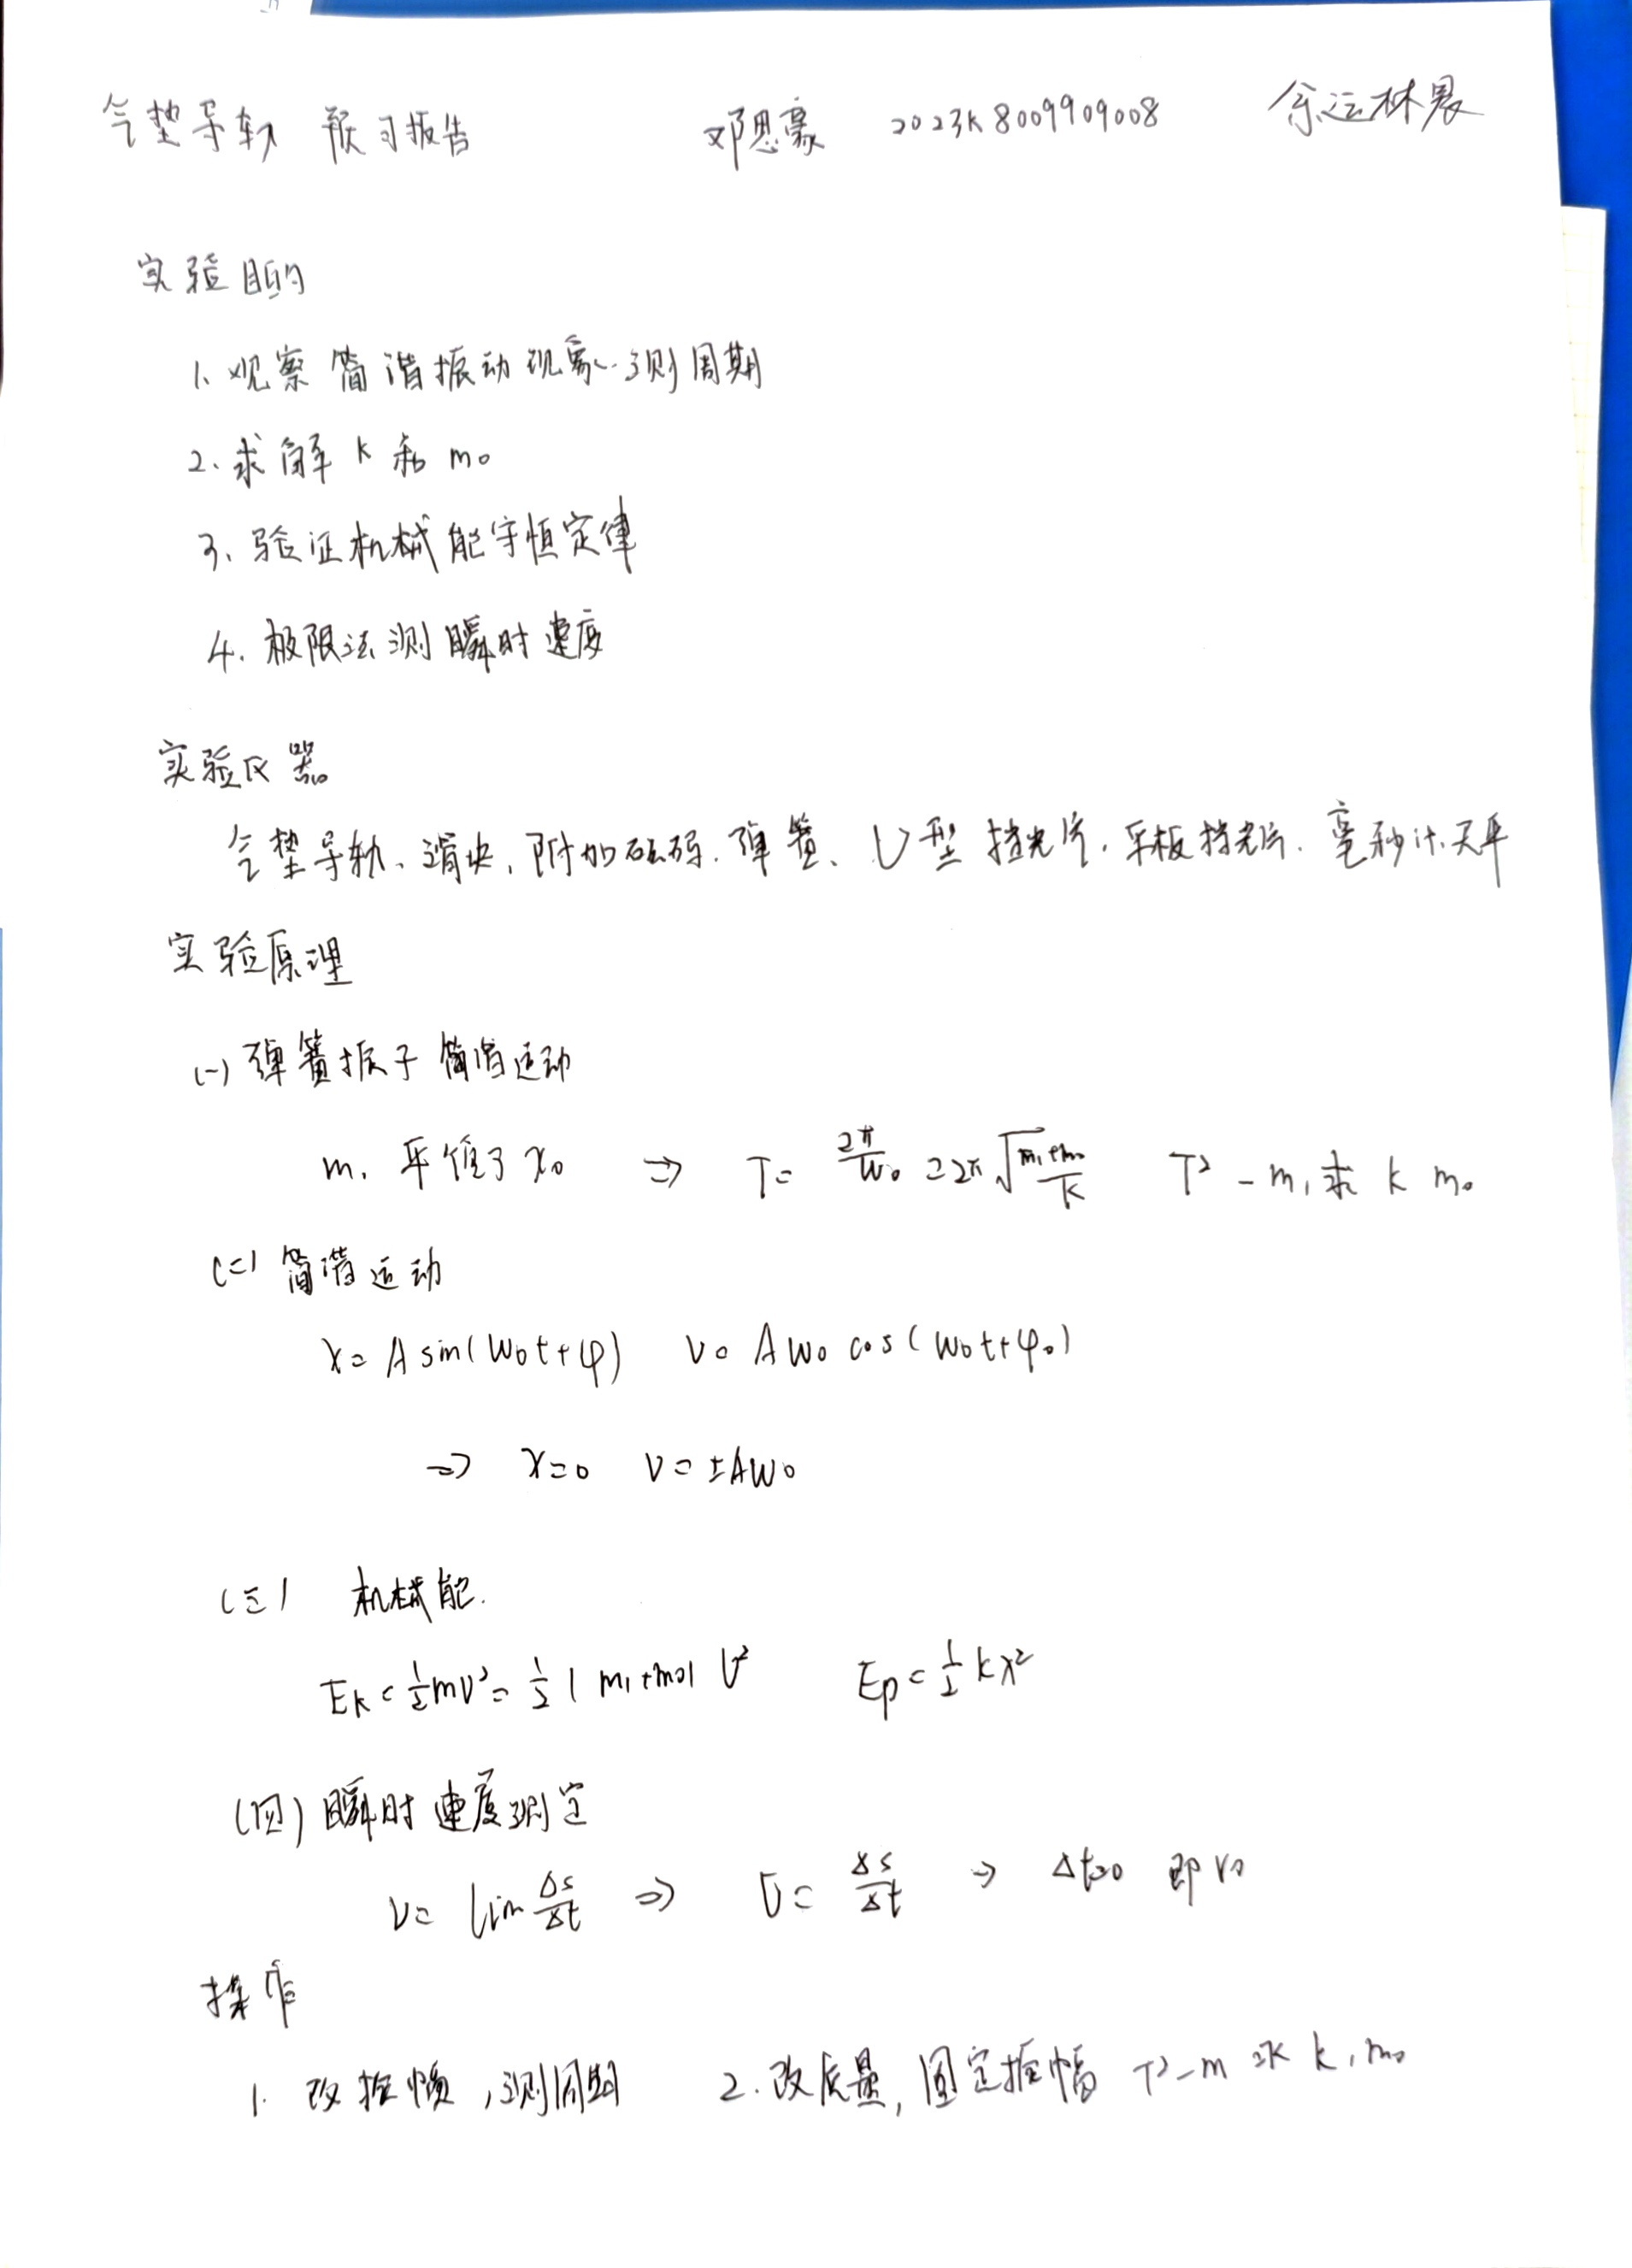
\includegraphics[width=0.98\textwidth]{record_pre.jpg}
\end{figure}

\begin{figure}[H]
    \centering
    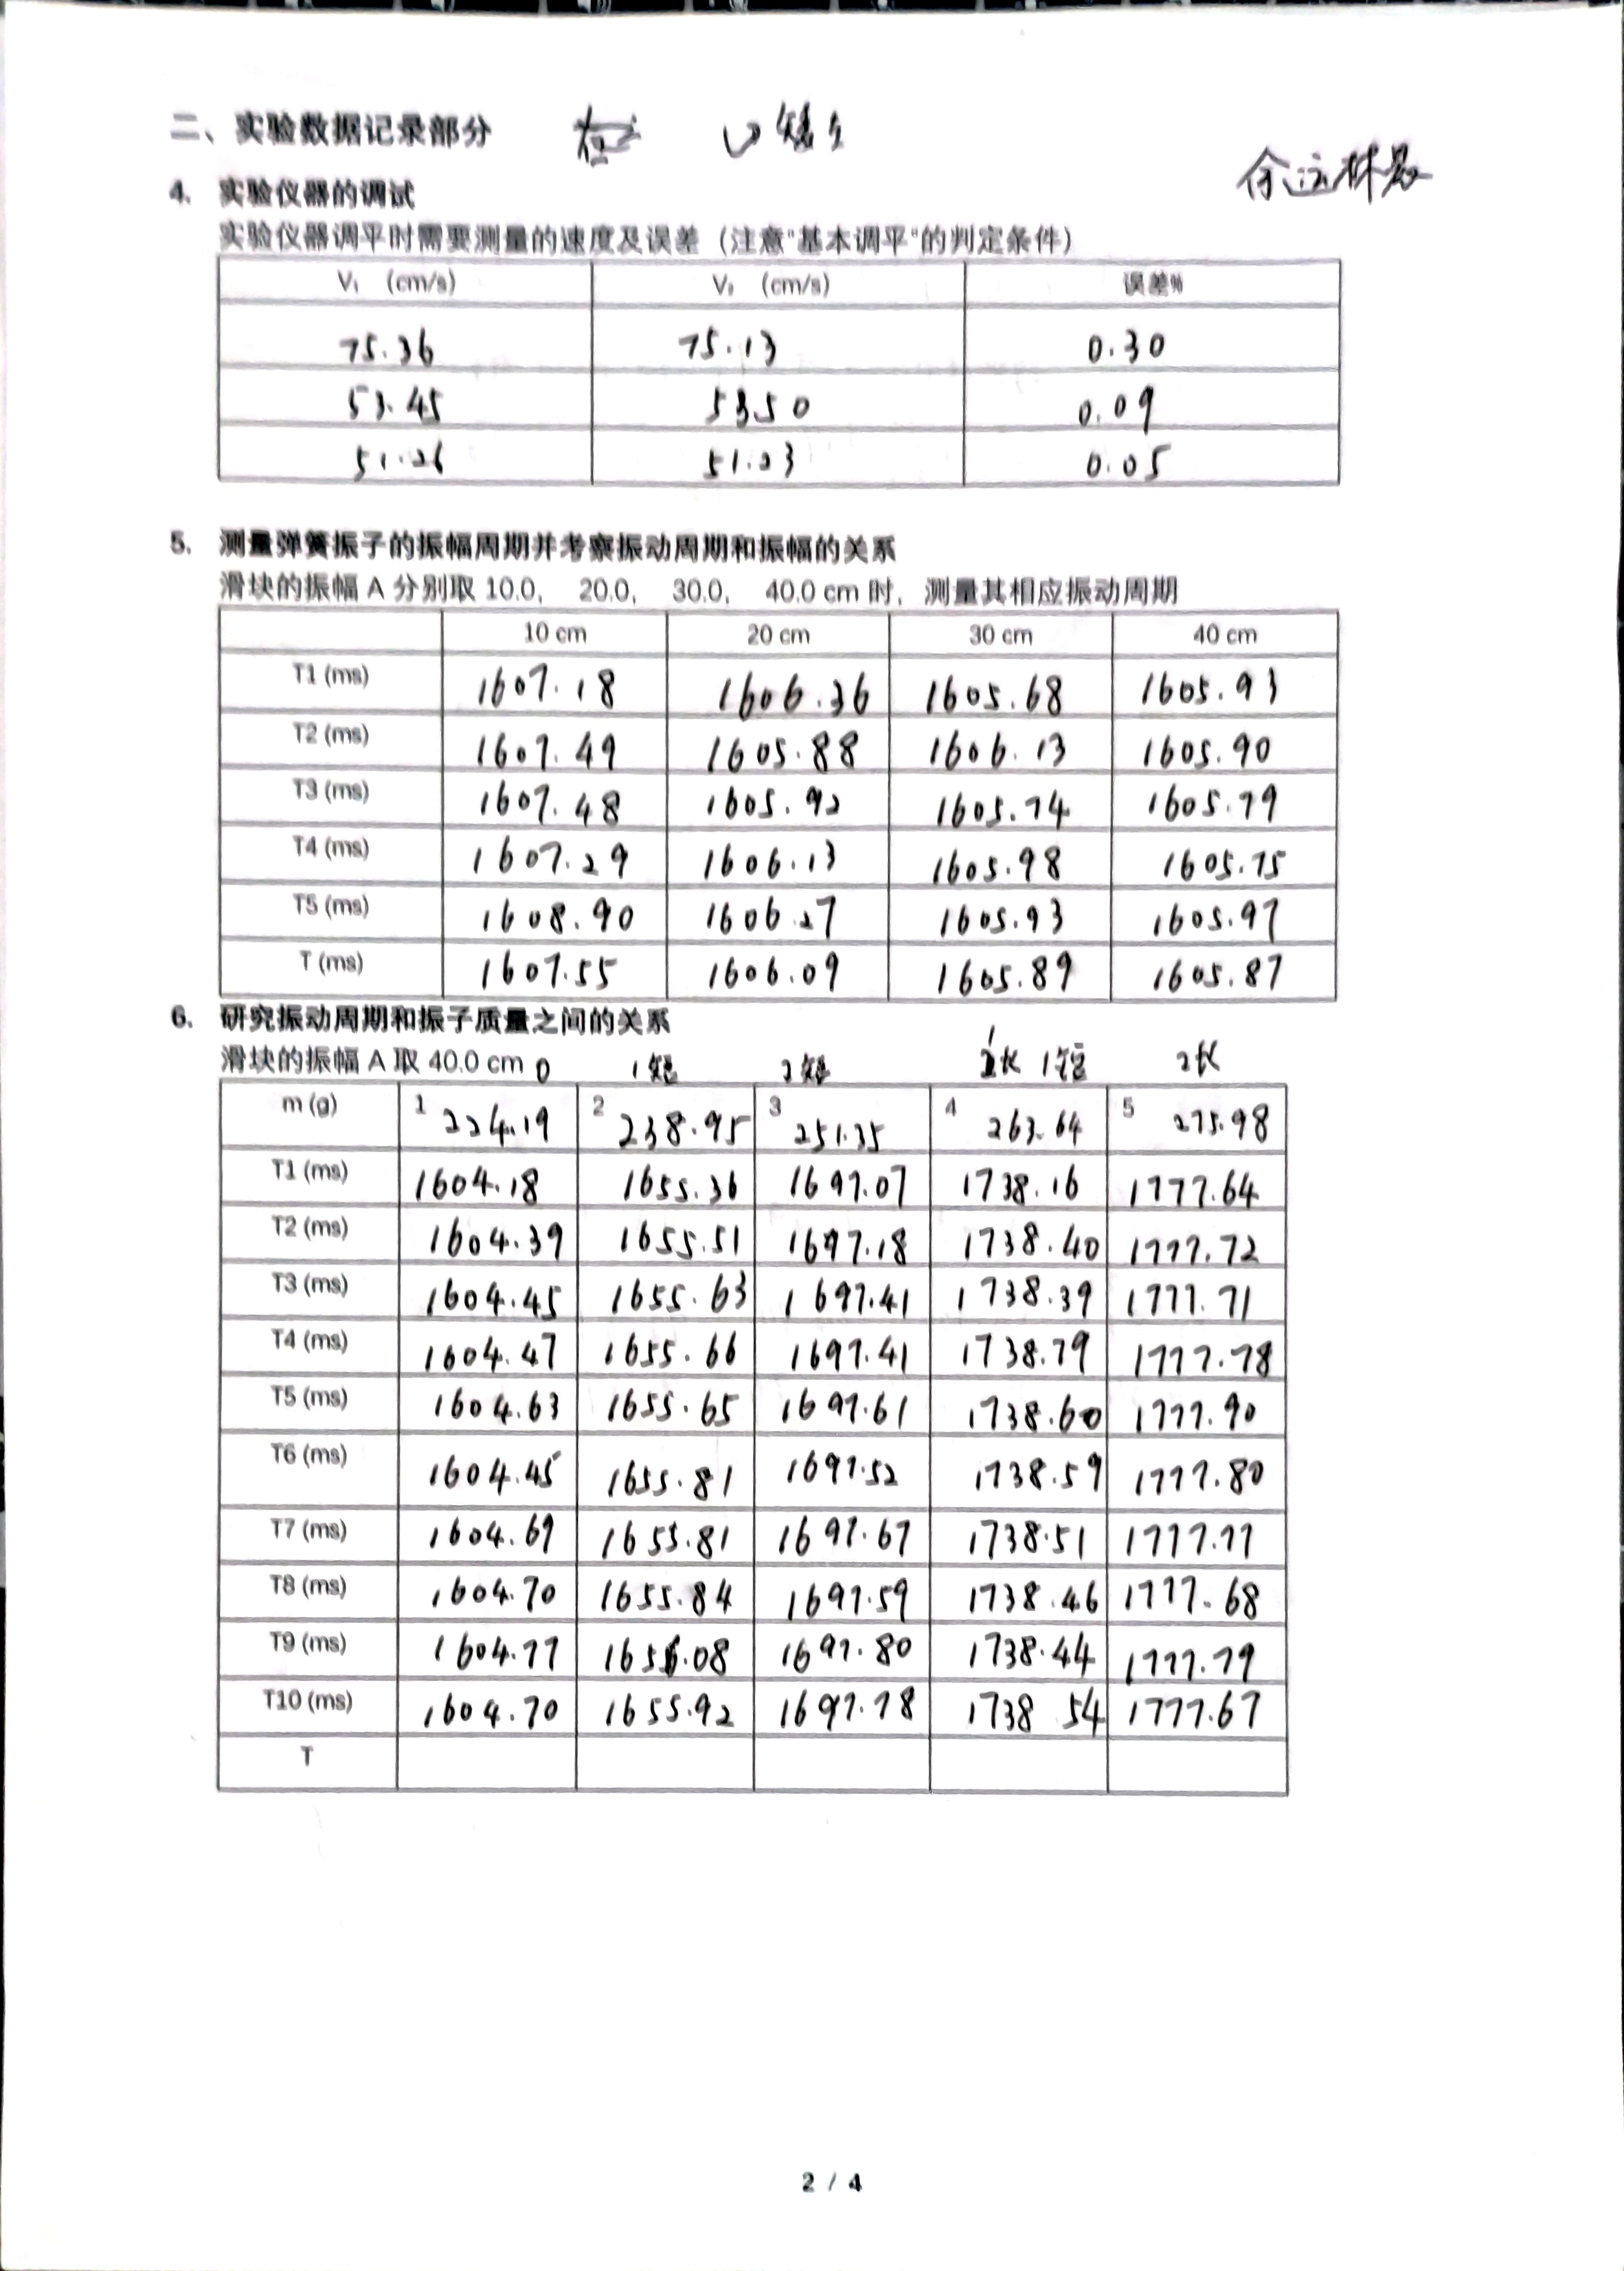
\includegraphics[width=0.98\textwidth]{record1.jpg}
\end{figure}

\begin{figure}[H]
    \centering
    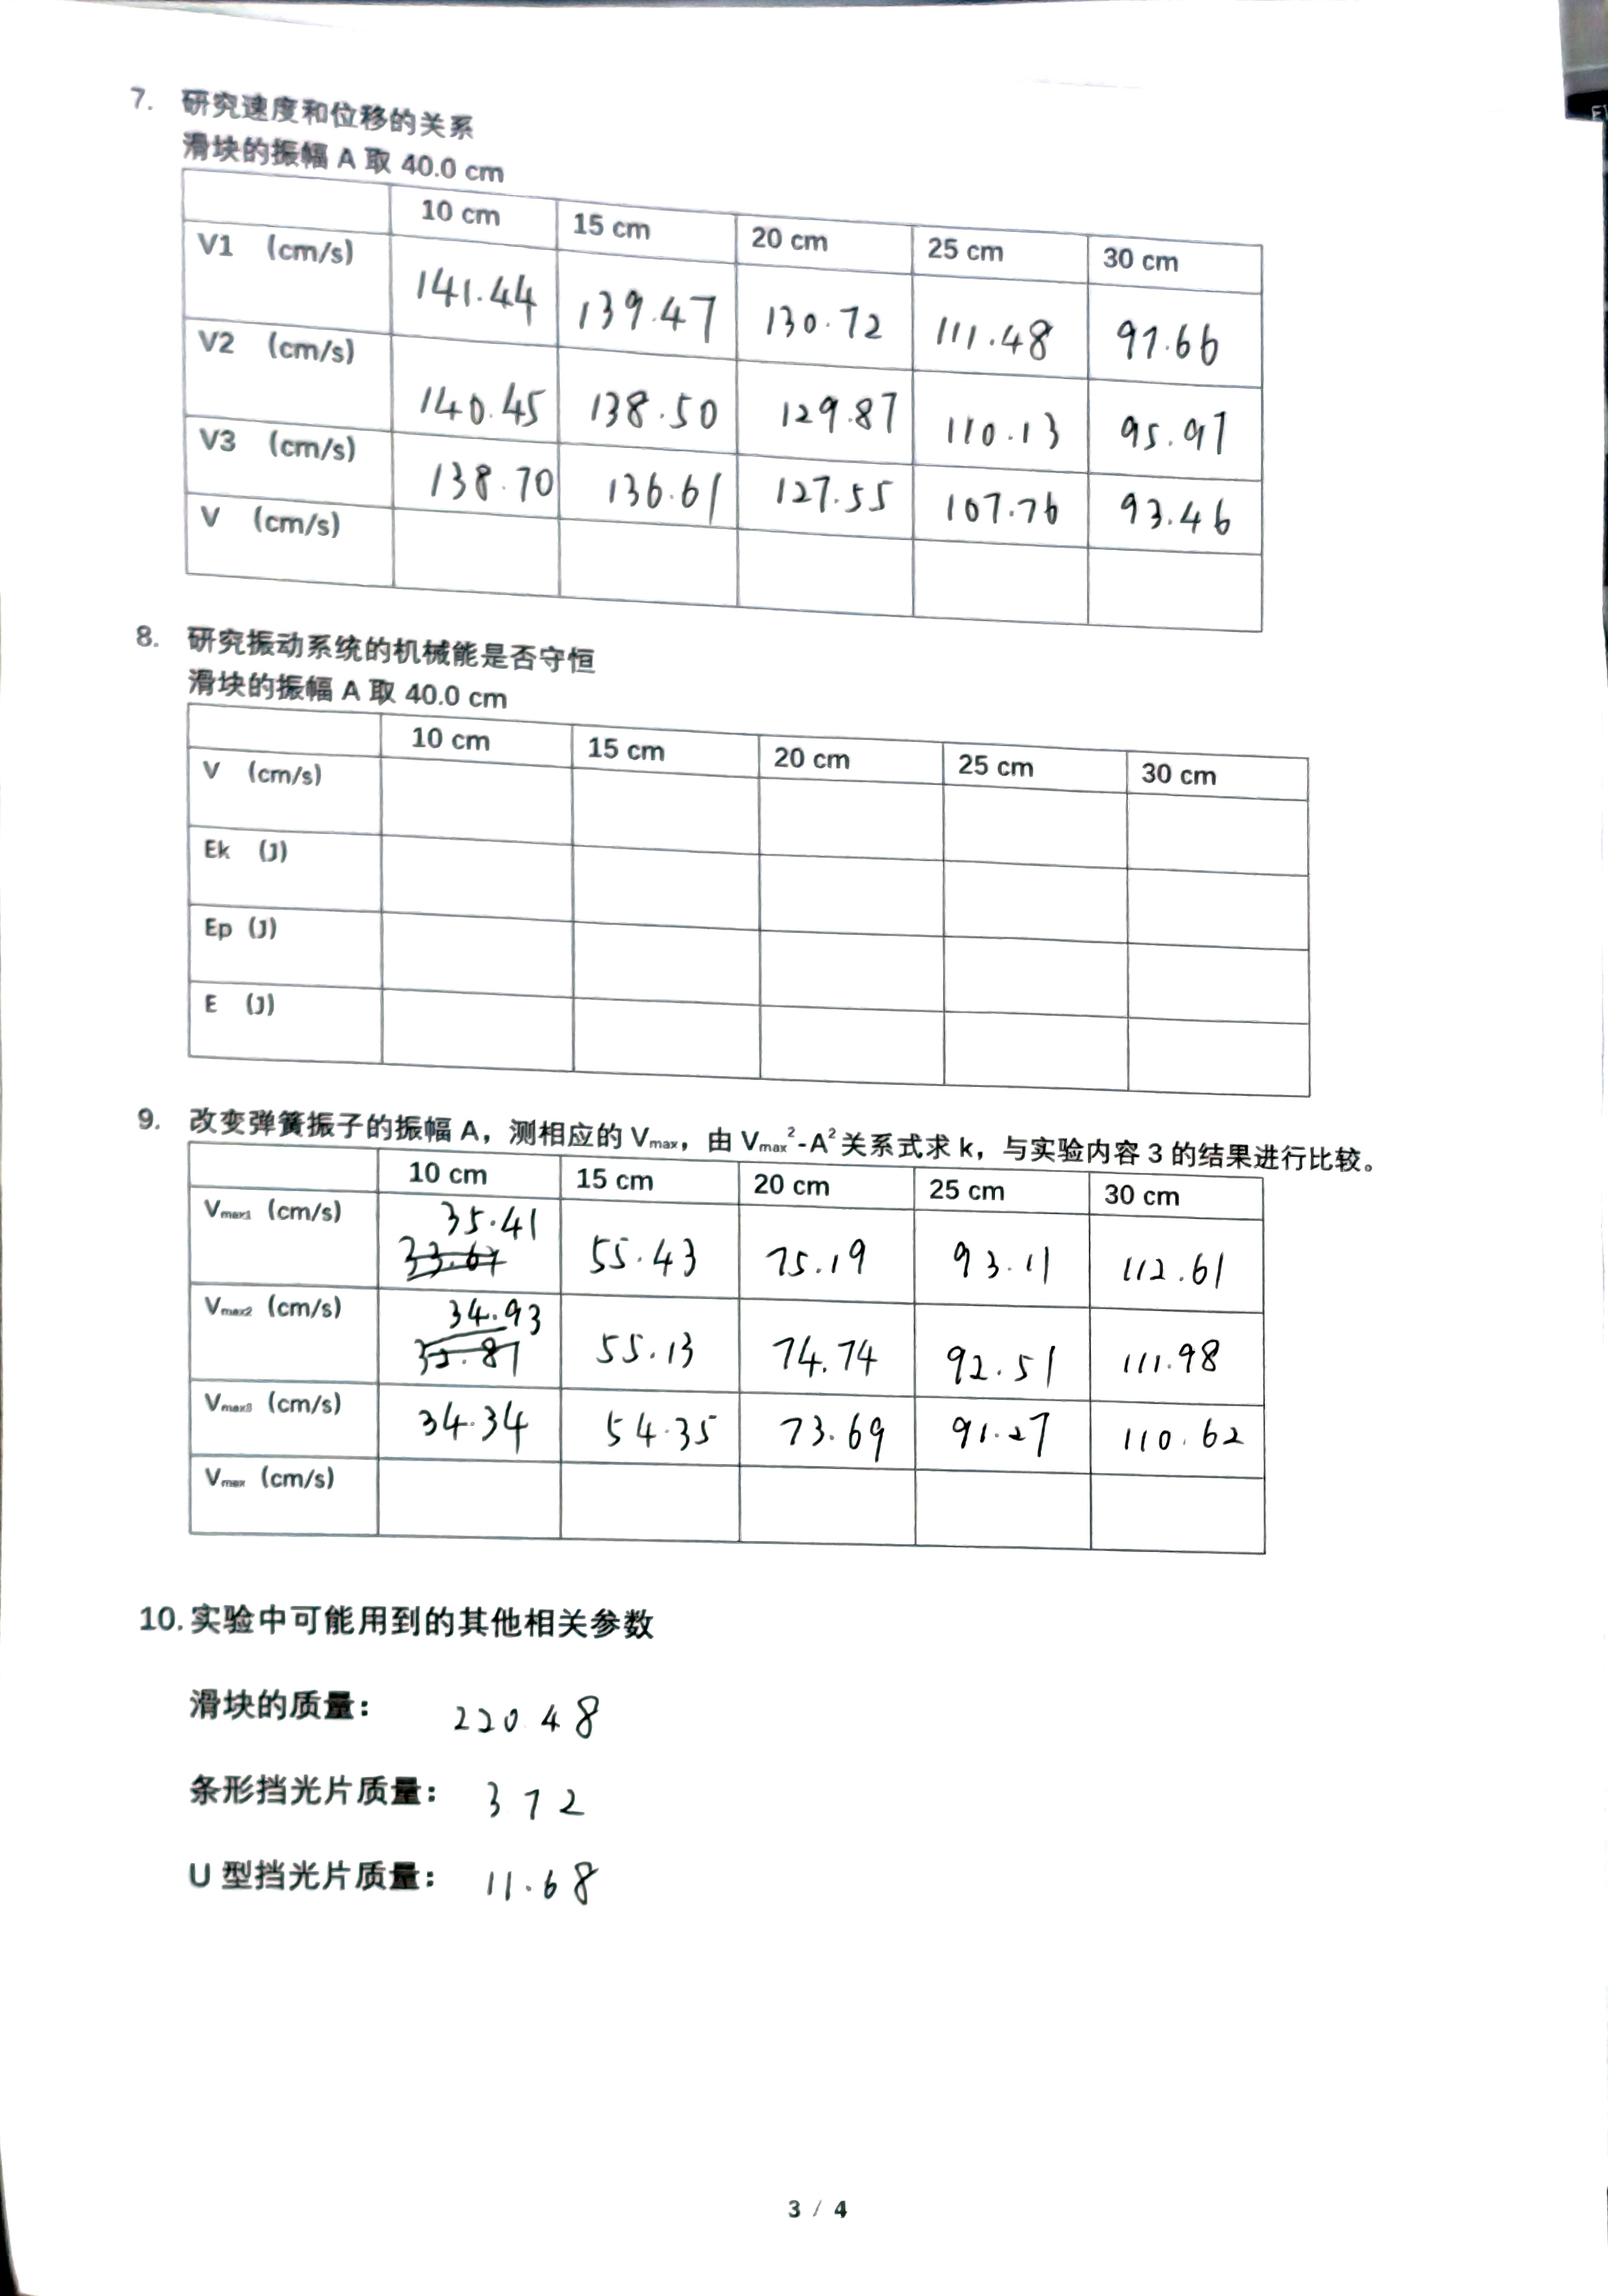
\includegraphics[width=0.98\textwidth]{record2.jpg}
\end{figure}

\begin{figure}[H]
    \centering
    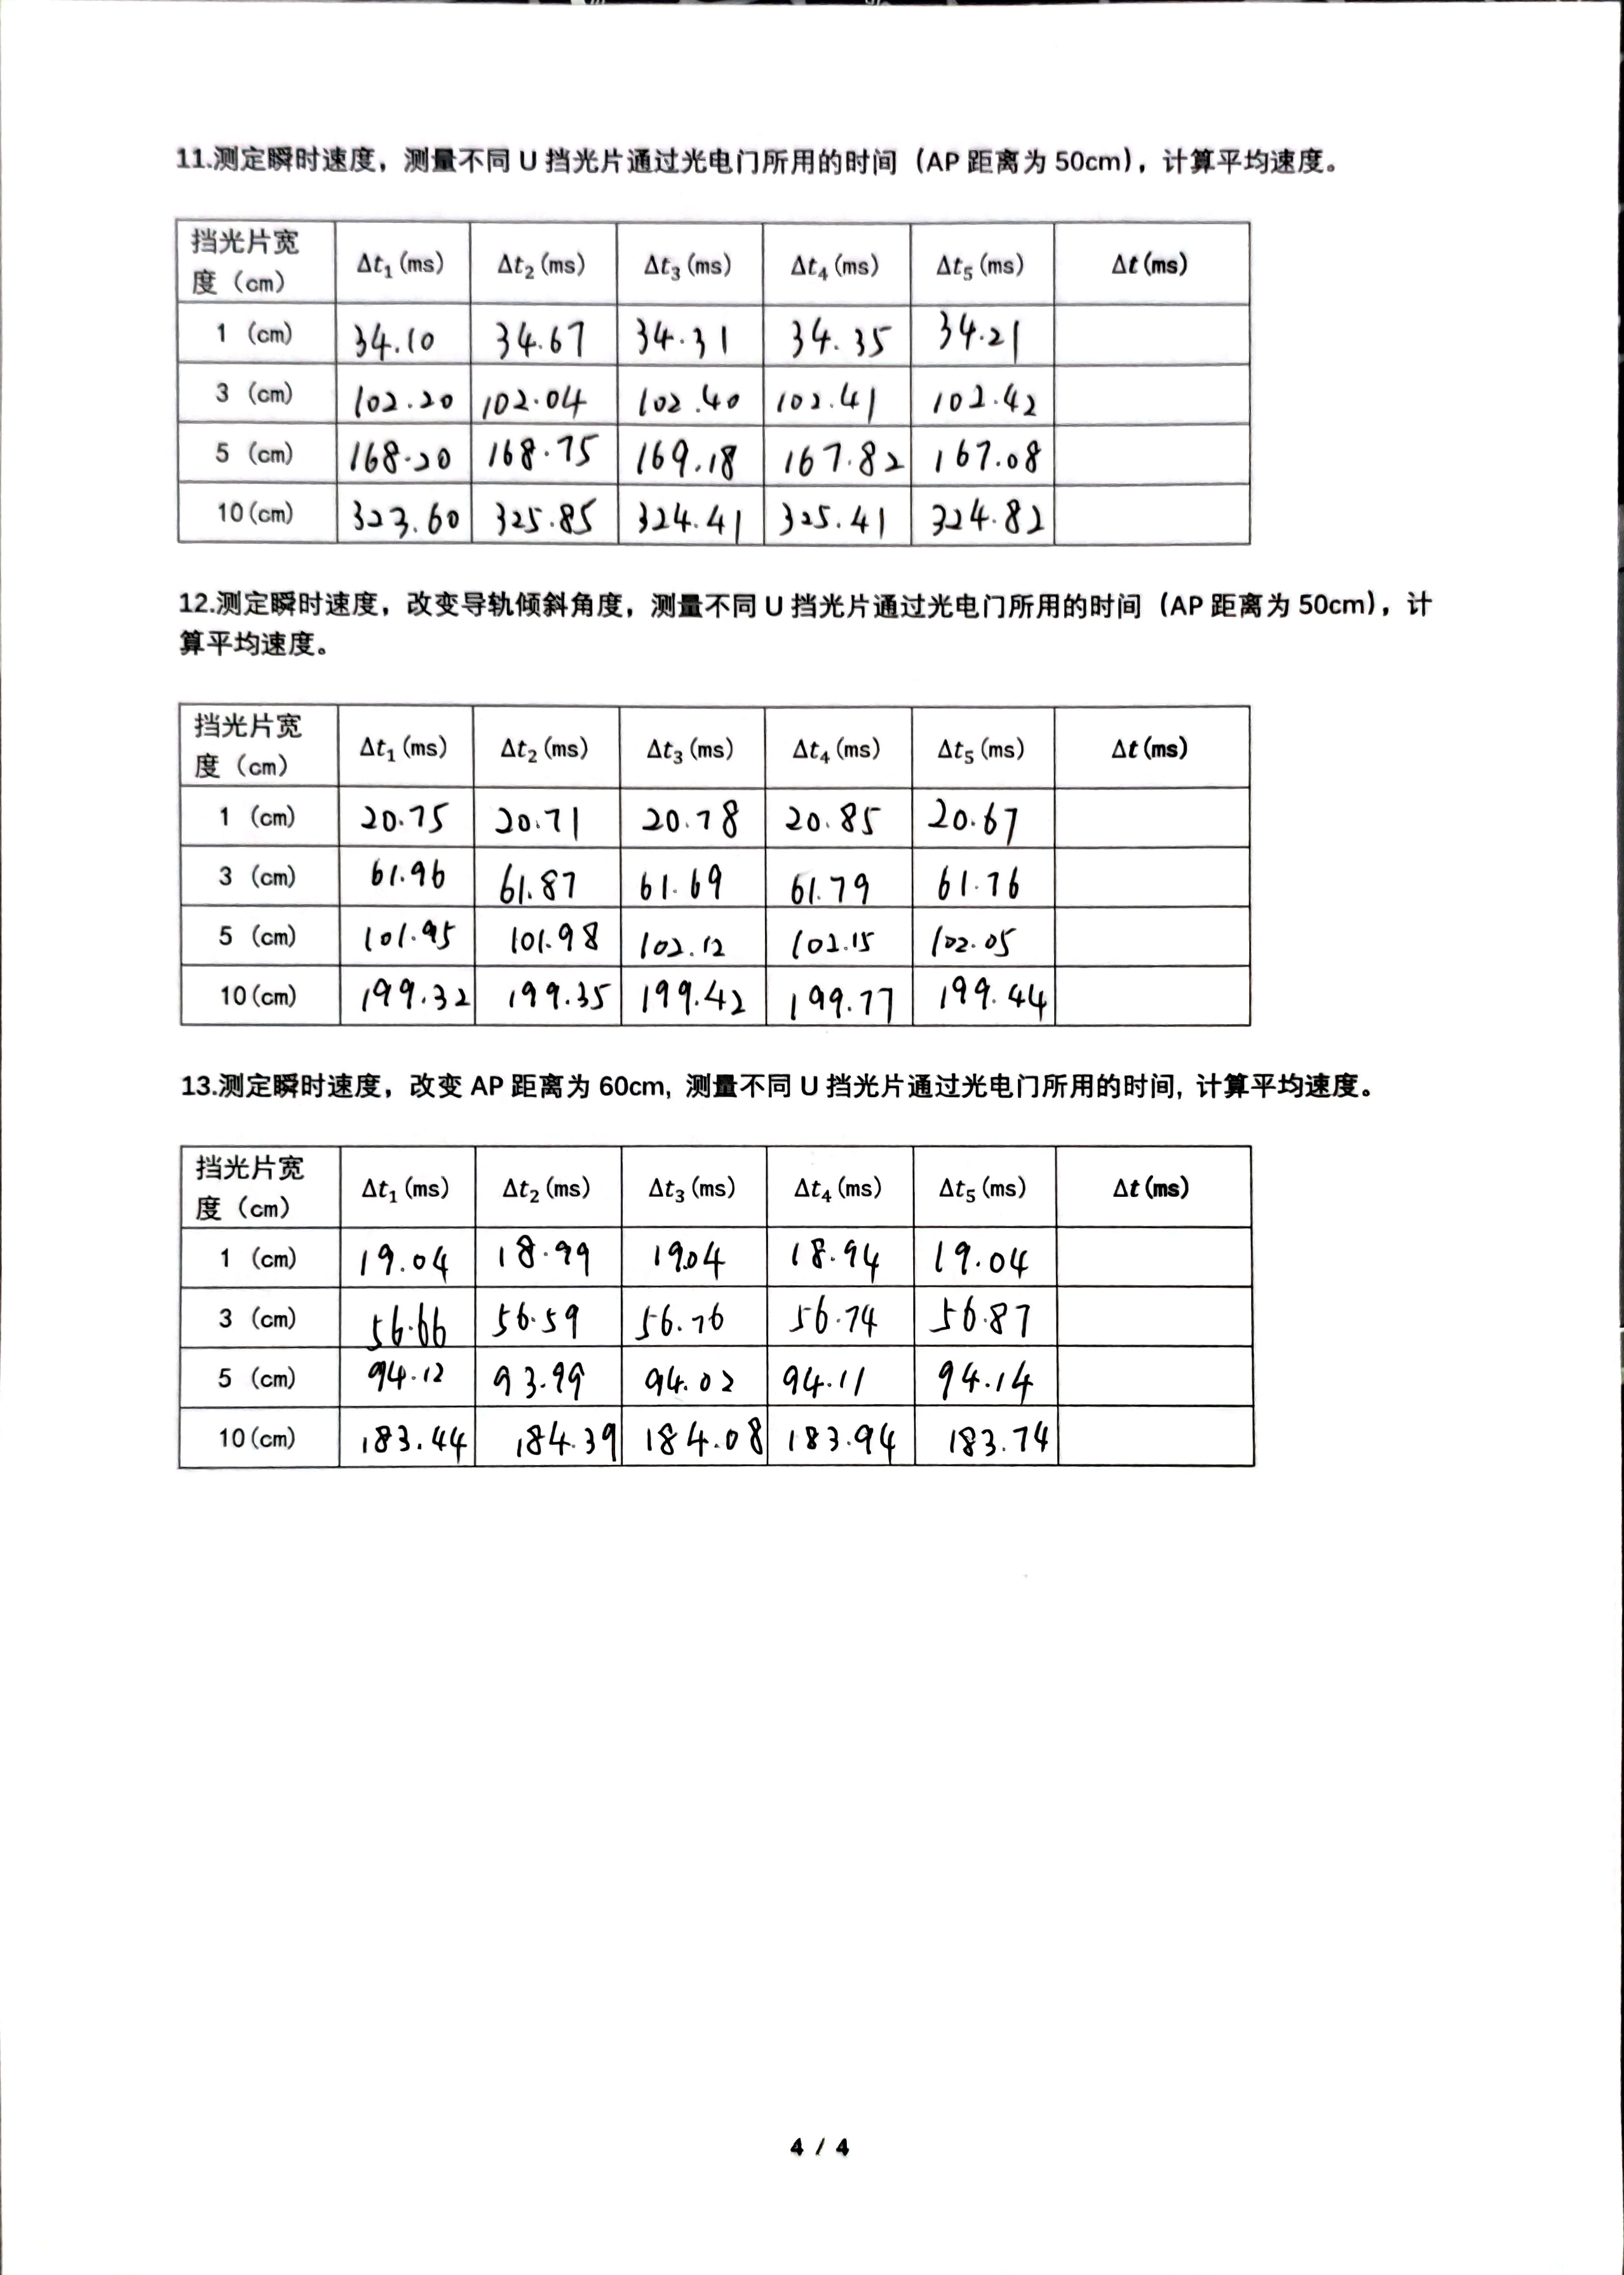
\includegraphics[width=0.98\textwidth]{record3.jpg}
\end{figure}

\end{document}